\documentclass[•]{beamer}
\usetheme{Rochester}

\usecolortheme[named=orange]{structure}
\setbeamercolor{block title alerted}{fg=white, bg=orange}

\begin{document}
	\begin{frame}
		\frametitle{The Factor Principle}
		- Turing proposed using a "factor principle" in cryptographic work.\\
		- Today, "factors" would be called Bayes Factors.\\
		- These were used to calculate a weight of evidence in favour of a given hypothesis (and were typically expressed in decihartleys (dHarts), which were referred to as decibans (dbans) at Bletchley Park.\\
		- The paper can be at \url{https://arxiv.org/abs/1505.04714}.\\
	\end{frame}
	\begin{frame}
		\frametitle{A Note on Bayes Factors I.}
		- A Bayes factor, $\mathcal{K}$, is caluclated as:
		$$\mathcal{K}_{10} = \frac{\mathcal{P}(D | M_{1})}{\mathcal{P}(D | M_{0})}$$
		- $\mathcal{P}(D | M_{i})$ is the marginal likelihood of a model-level expression of Bayes' theroem, \textit{i.e.},
		$$\mathcal{P}(M_{x} | D) = \frac{\mathcal{P}(D | M_{x}) \mathcal{P}(M_{x})}{\sum\limits_{j=1}^{n} \mathcal{P}(D | M_{j}) \mathcal{P}(M_{j})}$$
		where there are $n$ competing models.
	\end{frame}
	\begin{frame}
		\frametitle{A Note on Bayes Factors II.}
		The likelihood used in a Bayes factor is not the denominator from a parameter-level implementation of Bayes' theorem, \textit{i.e.},
		$$\mathcal{P}(\theta_{1} | D, M_{1}) = \frac{\mathcal{P}(D | \theta_{1}, M_{1})\mathcal{P}(\theta_{1} | M_{1})}{\int \mathcal{P}(D | \theta_{1}, M_{1})\mathcal{P}(\theta_{1} | M_{1}) d \theta_{1}}$$
		where $\mathcal{P}(D | M_{1}) = \int \mathcal{P}(D | \theta_{1}, M_{1})\mathcal{P}(\theta_{1} | M_{1}) d \theta_{1}$ as this marginalises over the (model) parameters $\theta$, not the models themselves.\\
	\end{frame}
	\begin{frame}
		\frametitle{Heart Failure: preamble}
		- In the paper, Turing gives some (fictitious) probabilities:
		\begin{alertblock}{\textbf{Prior information}}
					- $\frac{1}{5}$ die of heart failure\\
					- $\frac{2}{3}$ who die of heart failure die in bed\\
		- $\frac{1}{4}$ who die of other causes die in bed\\
		\end{alertblock}
		- \textbf{What is the probability someone died of heart failure having been found dead in bed?}
	\end{frame}
	\begin{frame}
		\frametitle{Heart Failure: worked example I.}
		- Recall Bayes' theorem: $$\mathcal{P}(H | B) = \frac{\mathcal{P}(B | H) \mathcal{P}(H)}{\mathcal{P}(B)}$$
		with $H$ as died of heart failure and $B$ in bed. As there are two discrete outcomes (heart failure death or not), $$\mathcal{P}(H | B) = \frac{\mathcal{P}(B | H) \mathcal{P}(H)}{\mathcal{P}(B | H) \mathcal{P}(H) + \mathcal{P}(B | \neg H) \mathcal{P}(\neg H)}$$
		- This can be calculated from the provided prior information\ldots\\
	\end{frame}
	\begin{frame}
		\frametitle{Heart Failure: worked example II.}
		\begin{align*}
			\mathcal{P}(H | B) = \frac{\frac{2}{3} \cdot \frac{1}{5}}{\frac{2}{3} \cdot \frac{1}{5} + \frac{1}{4} \cdot (1 - \frac{1}{5})}\\
			\mathcal{P}(H | B) = 0.4
		\end{align*}
	\end{frame}
	\begin{frame}
		\frametitle{Heart Failure: worked example III.}
		- Alternatively, this can be expressed as odds. Recall for generic hypothesis, $H$, and evidence , $E$, $$\mathcal{O}(H | E) = \frac{\mathcal{P}(H | E)}{\mathcal{P}(\neg H | E)}$$,
		and $$\mathcal{P}(H | E) = \frac{\mathcal{O}(H | E)}{1 + \mathcal{O}(H | E)}$$
	\end{frame}
	\begin{frame}
		\frametitle{Heart Failure: worked example IV.}
		- So, $$\mathcal{O}(H | B) = \mathcal{O}(B | H) \mathcal{O}(H)$$ 
		$$\therefore \mathcal{O}(H | B) = \frac{(\frac{2}{3})}{(\frac{1}{4})} \cdot \frac{(\frac{1}{5})}{(1 - \frac{1}{5})}$$
		$$\mathcal{O}(H | B) = \frac{2}{3}$$,
		$$\therefore \mathcal{P}(H | B) = \frac{\frac{2}{3}}{1 + \frac{2}{3}}$$
		$$\mathcal{P}(H | B) = 0.4$$
	\end{frame}
	\begin{frame}
		\frametitle{Heart Failure: code}
			- This example can also be carried out in Python and using a Bayesian network.\\
			- A Bayesian network is a more general forumlation of what Turing was taking about in the paper, and it makes generalising these calculations to the case when evidence is dependent on each other much easier.\\
			\begin{center}
				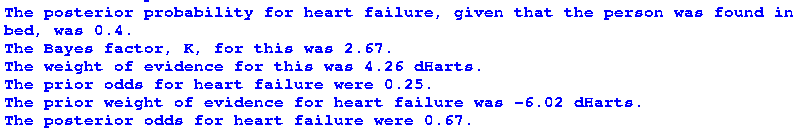
\includegraphics[width=10cm]{images/heart_py.png}\\
			\end{center}
			- See heart.py.
	\end{frame}
	\begin{frame}
		\frametitle{Interpreting Bayes Factors}
	\end{frame}
	\begin{frame}
		\frametitle{Appendix: deriving Bayes' theorem}
		- Starting with the idea of having an hypothesis, $H$, and some evidence $E$, what is the probability of $H$, given $E$ (\textit{i.e.}, $\mathcal{P}(H | E))$?\\
		- From the chain rule of probability (\url{https://en.wikipedia.org/wiki/Chain_rule_(probability)}), we have: $$\mathcal{P}(H \land E) = P(E | H) P(H)$$, and alternatively, $$\mathcal{P}(H \land E) = P(H | E) P(E)$$
		$$\therefore \mathcal{P}(H | E) = \frac{\mathcal{P}(H) \mathcal{P}(E | H)}{\mathcal{P}(E)})$$
	\end{frame}
\end{document}	